\section{L'ordonnancement cumulatif}
\label{sec:cumu}

\subsection{L'ordonnancement en programmation par contrainte}
\label{sec:cumu_ordo}

Les problèmes d'ordonnancement étudiés en programmation par
contraintes sont majoritairement regroupés en trois catégories: les
problème préemptifs, les problèmes non préemptifs et les problèmes
élastiques. Les problèmes préemptifs, respectivement non préemptifs,
sont des problèmes pour lesquels la préemption des activités est
autorisée, respectivement non autorisée. Une définition d'une activité
préemptive peut être trouvée dans le paragraphe~\ref{sec:ordo}. Les
{\it problèmes d'ordonnancement élastiques} correspondent aux
problèmes où la quantité de ressource attribuée à une activité peut
varier, à tout instant $t$ de l'horizon de temps, avec la contrainte
que la quantité totale de ressource consommée par l'activité durant
son exécution soit égale à une certaine valeur appelée {\it
  énergie}. Cette dernière notion peut aisément être étendue dans le
cas où l'énergie reçue par une activité n'est pas égale à la quantité
de ressource consommée mais où des fonctions de rendement modélisent 
cette conversion. Clairement, le \CECSP est un exemple typique d'un
tel problème. 

La majorité des problèmes d'ordonnancement non-préemptifs classiques
peuvent être modélisés à l'aide d'un problème de satisfaction de
contraintes. En général, trois variables représentant respectivement
la date de début d'une activité, notée $st_i$, sa date de fin, notée
$et_i$ et sa durée, notée $p_i$, sont définies. Les domaines de
chacune de ces variables sont définis par les données du problème. En
effet, pour chaque activité, nous pouvons calculer une date de début
au plus tôt, $\ES$, et au plus tard, $\LS$; ainsi, le domaine de la
variable $st_i$ est $[\ES,\LS]$. De même, le domaine de la variable
$et_i$ est $[\EE,\LE]$, avec $\EE$ la date de fin au plus tôt de $i$
et $\LE$ sa date de fin au plus tard. La durée d'une activité est
quant à elle définie comme la différence entre sa date de fin et sa
date de début, i.e. $p_i=et_i-st_i$.

Les problèmes préemptifs sont plus difficiles à modéliser. En effet,
dans ce cas-là, un ordonnancement valide ne peut seulement être
représenté par une date de début, de fin et une durée pour chaque
activité. Pour ces problèmes, au moins deux modélisations différentes
existent. La première consiste à associer à chaque activité une
variable d'ensemble, i.e. une variable dont la valeur sera un
ensemble. Cet variable représente l'ensemble des instants $t$ où
l'activité est en cours, définie comme un ensemble d'intervalles ou de
temps $t$ discret. Une second possibilité est de définir une variable
binaire, pour chaque activité et chaque instant $t$, qui prendra la
valeur $1$ si l'activité est en cours à l'instant $t$. Notons que,
dans le cas d'un problème d'ordonnancement continu, une telle solution
ne peut être envisageable car cela conduirait à un nombre infini de
telles variables.

Les problèmes élastiques sont, quant à eux modéliser, à travers les
contraintes de ressources. Il existe deux principaux types de
contraintes de ressource en PPC. Le premier permet de modéliser les
ressources disjonctives, i.e. qui ne peuvent exécuter qu'une activité
en parallèle, et le second sert à la modélisation des ressources
cumulatives. Ici, nous nous intéressons seulement au second cas.

{\'E}tant donné une activité et une ressource de capacité $R$, une
variable $b_i$ sert généralement à modéliser la consommation de
l'activité sur cette ressource. Dans le cas des tâches élastiques,
cette variable est remplacée par une variable $W_i$ représentant
l'énergie requise par l'activité. Pour représenter un ordonnancement,
un ensemble de variables représentant la quantité de ressource
utilisée par une activité à l'instant $t$ est introduit. Ces variables
sont ensuite liés entre elles par un ensemble de contraintes
modélisant le fait que chaque activité doit recevoir une énergie
$W_i$. 

Ces différents concepts peuvent être étendus pour modéliser d'autre
types de contraintes telles que des contraintes de ressources
alternatives, des temps de préparation entre les activités, des
activités optionnelles ou des contraintes de réservoirs.

Dans la suite de ce manuscrit, nous nous intéressons aux problèmes
d'ordonnancement non-préemptifs avec ressource cumulative et aux
problèmes d'ordonnancement élastiques. Le premier cas correspond au
\CUSP, décrit dans le paragraphe~\ref{sec:ordo_res}. En PPC, le
problème est modélisé à l'aide d'une contrainte globale appelées
contrainte cumulative. Cette contrainte ainsi que différents
algorithmes de filtrage mis en place pour cette dernière sont
présentés dans les deux paragraphes suivant. 

Les problèmes d'ordonnancement élastiques seront représentés par le
\CECSP~(voir paragraphe~\ref{sec:ordo_nrj}), pour lequel une partie
des algorithmes de filtrage pour la contrainte cumulative sont adaptés
et un modèle de PPC dans le cas de la restriction discrète du
\CECSP~seront présentés dans le chapitre~\ref{sec:PPC_CECSP}.

\subsection{La contrainte cumulative}
\label{sec:cumu_cume}

En PPC, le \CUSP~est modélisé par la contrainte cumulative. Dans ce
contexte, une activité est souvent représentée par $4$ variables:
$st_i,\ et_i,\ p_i$ et $b_i$ correspondant respectivement à la date de
début de l'activité, sa date de fin, sa durée et sa consommation de
ressource. En règle générale, les domaines des variables $p_i$ et
$b_i$ sont restreint à un seul élément, i.e. la durée de l'activité
est fixe et sa consommation de ressource est constante durant toute
son exécution. 

La contrainte cumulative vise donc à déterminer seulement les dates de
début et de fin des activités -- liés par la condition d'intégrité
$et_i=st_i+p_i$. Cette contrainte prend donc en paramètre l'ensemble
d'activités $\A$ à ordonnancer et la capacité $R$ de la ressource utilisée
pour exécuter les activités. Avec ces notations la contrainte s'écrit
$cumulative(\A,R)$ et cette contrainte est satisfaites si et seulement 
si:
\begin{align}
  \forall i \in \A, & \quad  st_i+p_i=et_i \label{eq:CUSP_int}\\
  \forall t \in \H, &\quad \sum_{\substack{i \in A\\t \in
  [st_i,et_i[}} b_i \le R  \tag{\ref{eq:CUSP_res}} 
\end{align}
La seconde contrainte ainsi qu'un exemple de solution sont détaillés
dans le paragraphe~\ref{sec:ordo_res}.

L'existence d'une solution au problème cumulatif étant NP-complet, un
algorithme effectuant un filtrage complet des domaines des variables,
i.e. retirant toutes les valeurs incohérentes des domaine des
variables, ne peut s'exécuter en temps polynomial. De ce fait, les
algorithmes de filtrage se limite souvent à s'assurer de la cohérence
des bornes des domaines des variables. Ces algorithmes se présentent
le plus souvent sous la forme de règles permettant d'ajuster ces
bornes en fonction des données et contraintes du problème,
i.e. les {\it règles d'ajustement}. Malgré tout, ces techniques
restent encore trop coûteuse en temps pour être utilisées directement
sur la contrainte cumulative.  Différentes relaxations de la
contrainte cumulative ont donc été introduites et des règles
d'ajustement pouvant être appliquées en temps polynomial ont été mis
en place pour ces relaxations.

Baptiste {\it et al.}~\cite{BLPN} présentent un panorama de ces
différentes relaxations ainsi que des principales techniques issues de
la programmation par contraintes mis en place pour résoudre la
contrainte cumulative. Dans un contexte plus général, Dornoff {\it et
al.}~\cite{DHP} exhibent des règles de cohérence basées sur la
capacité des intervalles, i.e. la quantité de ressource disponible
dans un intervalle.

Le paragraphe suivant présente plusieurs des règles d'ajustement
définies pour la contrainte cumulative. 


\subsection{Les filtrages de la contrainte cumulative}
\label{sec:cumu_propag}

Le problème cumulatif étant un problème symétrique, les règles
d'ajustement sont souvent définie pour une seule des deux variables
$st_i$ et $et_i$. En effet, une fois ces règles définies pour une de
ces deux variables, les même règles peuvent être définies dans l'autre
cas de manière vraiment similaire. De ce fait, les raisonnements et
algorithmes décrit dans ce paragraphe ne présentent que le filtrage du
début au plus tôt.

Dans un premier temps, nous présentons des règles simples permettant
l'ajustement des bornes des variables. Ensuite, une partie sera
consacrée aux règles d'ajustement basée sur le concept
d'énergie. Enfin, ces règles seront ensuite combinées afin de créer
des algorithmes permettant un filtrage plus fort des domaines des
variables.

Plusieurs des règles présentées dans cette section seront ensuite
adaptées dans le cas du \CECSP~dans le chapitre~\ref{sec:PPC_CECSP}.

\subsubsection{Règles de filtrages simples}

Parmi les raisonnements les plus simples appliqués dans le cadre de la
contrainte cumulative, on retrouve le Time-Table~\cite{TTLah} et le
raisonnement disjonctif~\cite{BLPN}.  

\paragraph{Time-Table}
Le premier algorithme de filtrage de la contrainte cumulative
présenté est basé sur la notion de {\it partie obligatoire} d'une
activité. Cette partie obligatoire correspond à l'intervalle de temps
maximal pendant lequel on est sûr que l'activité devra être
exécutée. Cet intervalle est vide dans le cas où $\LS \ge \EE$, et est
égal à $[\LS,\EE{[}$ dans le cas contraire. Notons que dans le cas de la
contrainte cumulative, une borne supérieure sur la date de début d'une
activité peut aisément être calculée. En effet, il suffit de prendre
$\LS=\LE - p_i$. 


\begin{defi}
La partie obligatoire d'une activité $i$ est l'intervalle $[\LS,\EE{[}$.
\end{defi}

\begin{ex}
Considérons l'activité suivante: 

\vspace{-0.5cm}
\begin{center}
  \begin{tabular}{|P{1cm}P{1cm}P{1cm}P{1cm}|}
    \hline
    \ES & \LE & p_i & b_i  \\
    \hline
    1 & 13 & 8 & 2 \\
    \hline
  \end{tabular}
\end{center}

Nous pouvons calculer sa date de début au plus tard,
$\LS=\LE - p_i=13-8=5$, ainsi que sa date de fin au
plus tôt, $\EE=\ES + p_i=1+8=9$. Comme $\EE > \LS$,
l'activité possède une partie obligatoire qui est l'intervalle $[5,9[$
(voir figure~\ref{fig_mand_CUSP}).
  
\begin{figure}[htb!]
\subcaptionbox{Ordonnancement au plus tôt}[0.3\linewidth]{
    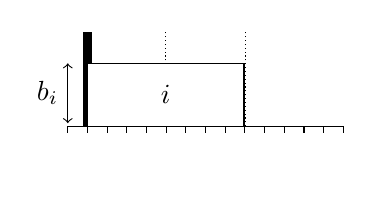
\begin{tikzpicture}
      [xscale=0.25, yscale= 0.4,node distance=0.5cm]
      \node (sil) at (1,0) {} ;
      \node (eil) at (9,0) {} ;
      \node [below of=eil,node distance=0.63cm]  {$\EE$};
      \draw (sil.center) node[below=0.2cm] {$\ES$};
   \node (sir) at (5,0) {} ;
      \node (eir) at (13,0) {} ;
      \node[below of= sir,node distance=0.63cm] {$\LS$};
      \draw (eir.center) node[below=0.2cm] {$\LE$};
      
      \draw (0,0) -- (14,0);
      \draw[line width=3pt] (1,0) -- (1,3);
      
      \draw[densely dotted] (9.05,0) -- (9.05,3);
     \draw[densely dotted] (4.95,0) -- (4.95,3);
      \draw[<->] (0,0.1) -- (0,2) node[midway,left] {$b_i$};
      \draw[fill=white] (1,0) rectangle (8.95,2) node[midway] {$i$};

      \foreach \i in {0,...,14} {
        \draw (\i,0)  -- (\i,-0.2);
      }
    \end{tikzpicture}
}
\hfill
\subcaptionbox{Ordonnancement au plus tard}[0.3\linewidth]{
    \begin{tikzpicture}
      [xscale=0.25, yscale= 0.4,node distance=0.5cm]
        \node (sil) at (1,0) {} ;
      \node (eil) at (9,0) {} ;
      \node [below of=eil,node distance=0.63cm]  {$\EE$};
      \draw (sil.center) node[below=0.2cm] {$\ES$};
   \node (sir) at (5,0) {} ;
      \node (eir) at (13,0) {} ;
      \node[below of= sir,node distance=0.63cm] {$\LS$};
      \draw (eir.center) node[below=0.2cm] {$\LE$};
      
      \draw (0,0) -- (14,0);
      \draw[line width=3pt] (13,0) -- (13,3);
      
      \draw[densely dotted] (4.95,0) -- (4.95,3);
      \draw[densely dotted] (9.05,0) -- (9.05,3);
      \draw[<->] (14,0.1) -- (14,2) node[midway,right] {$b_i$};
      \draw[fill=white] (5.05,0) rectangle (13,2) node[midway] {$i$};

      \foreach \i in {0,...,14} {
        \draw (\i,0)  -- (\i,-0.2);
      }
    \end{tikzpicture}
}
\hfill
\subcaptionbox{Partie obligatoire}[0.3\linewidth]{ 
  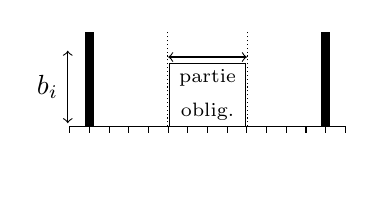
\begin{tikzpicture}
    [xscale=0.25, yscale= 0.4,node distance=0.5cm]
    \node (sir) at (5,0) {} ;
    \node (eil) at (9,0) {} ;
    \node [below of=eil,node distance=0.63cm]  {$\EE$};
    \node[below of= sir,node distance=0.63cm] {$\LS$};
    \draw[<->] (5,2.2) -- (9,2.2) node[midway,label={}]
    {};
    
    \draw (5.05,0) rectangle (8.95,2)
    node[midway,color=black,align=center,text width=1.4cm]
    {\scriptsize partie oblig.}; 
    
    
    \draw (0,0) -- (14,0);
    \draw[line width=3pt] (1,0) -- (1,3);
    \draw[line width=3pt] (13,0) -- (13,3);
    
    \draw[<->] (-0.1,0.1) -- (-0.1,2.4) node[midway,left] {$b_i$};

    \draw[densely dotted] (4.95,0) -- (4.95,3);
    \draw[densely dotted] (9.05 ,0) -- (9.05,3);

    \foreach \i in {0,...,14} {
      \draw (\i,0)  -- (\i,-0.2);
    }
  \end{tikzpicture}
}
\caption{Partie obligatoire d'une activité $i$}
\label{fig_mand_CUSP}
\end{figure}
\end{ex}

Le profil obligatoire des activités peut ensuite être agrégé de
manière à obtenir une fonction en escalier, appelée {\it profil
  obligatoire de la ressource}.  

\begin{defi}
  Le {\bf profil obligatoire} d'une ressource $TT_{\cal A}$ est définie
  par la fonction suivante: $TT_{\cal A}(t)= \sum_{\substack{i \in {\cal
        A}\\ \LS \le t < \EE}} b_i ,\ \forall t \in \H$.  Le problème n'admet
  pas de solution si $\exists t \in \H \ : \ TT_{\cal A}(t) > R$.
\end{defi}


\begin{ex}
  \begin{figure}[!htb]
    \centering
    \begin{tikzpicture}
      [yscale=0.45,xscale=0.6]
      \node (O) at (0,0) {};
      \foreach \i in {0,...,13} {
        \draw (\i-1,0) -- (\i-1,-0.1) node[below] {$\i$};
      }
      
      \draw (0,0) -- (0,2) -- (2,2) -- (2,4) -- (4,4) -- (4,6) --
      (5,6) -- (5,1) -- (9,1) -- (9,3) -- (11,3) -- (11,0);
      \draw[->] (-1,0) -- (12.5,0);
      \draw[dashed] (-1,5) -- (12.5,5);
      \draw[->] (-1,0) -- (-1,5.5) node[left] {$R=5$};
    \end{tikzpicture}
    \caption{Exemple de profil obligatoire d'une ressource}
    \label{fig_profil_CUSP}
  \end{figure}
  Dans l'exemple décrit par la figure~\ref{fig_profil_CUSP}, nous
  remarquons que, au temps $t=1$, le profil obligatoire de la
  ressource vaut $2$. Comme la ressource est de capacité $5$, aucune
  incohérence n'est détectée. À l'inverse, au temps $t=5$, le profil
  obligatoire de la ressource a une valeur de $6$, ce qui est
  supérieur à la capacité de la ressource. Une incohérence est donc
  détectée et il n'existe pas de solution réalisable pour cette
  instance. 
\end{ex}

Pour réaliser un filtrage des bornes, nous devons fournir des règles
permettant d'identifier si débuter l'activité $i$ à $\ES$ (ou $\LS$)
ne viole pas les contraintes du problème. Cette règle peut être
formalisée de la façon suivante: 

\begin{reg}
\label{reg:TT}
Soit une activité $i \in \A$. S'il existe $t \in [\ES,\LS{[}$ tel que
$t < \EE$ et que $b_i + TT_{\A \setminus\{i\}}(t) > R$ alors la date
de début au plus tôt de $i$ peut être ajustée et on a: $ \ES > t$.
\end{reg}

\begin{ex}
 Soit l'activité définie ci-dessous.
\begin{center}
  \begin{tabular}{|P{1cm}P{1cm}P{1cm}P{1cm}|}
    \hline
    \ES & \LE & p_i & b_i  \\
    \hline
    1 & 14 & 8 & 2 \\
    \hline
  \end{tabular}
\end{center}
La figure~\ref{fig:TT_CUSP} présente le profil obligatoire de la
ressource ainsi que l'ajustement déduit de la règle~\ref{reg:TT}.
  \begin{figure}[!htb]
    \centering
    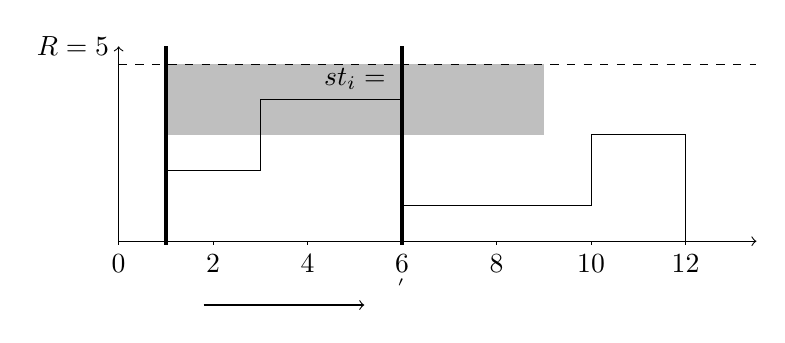
\begin{tikzpicture}
      [yscale=0.45,xscale=0.6]
      \node (O) at (0,0) {};
      \foreach \i in {0,2,...,13} {
        \draw (\i-1,0) -- (\i-1,-0.1) node[below] {$\i$};
      }
      
      \fill[draw=black,gray!50] (0,5) rectangle (8,3) node[midway,above,color=black]
      {$st_i=\ES$};
      \draw (0,0) -- (0,2) -- (2,2) -- (2,4) -- 
      (5,4) -- (5,1) -- (9,1) -- (9,3) -- (11,3) -- (11,0);
      \draw[->] (-1,0) -- (12.5,0);
      \draw[dashed] (-1,5) -- (12.5,5);
      \draw[->] (-1,0) -- (-1,5.5) node[left] {$R=5$};
      \draw[very thick=3pt] (0,-0.1) node[below=0.4cm] {$\ES$}-- (0,5.5);
      \draw[very thick=3pt] (5,-0.1) node[below=0.3cm] {$\ES^{'}$}-- (5,5.5);
      \draw[->] (0.8,-1.8) -- (4.2,-1.8);
    \end{tikzpicture}
    \caption{Règle d'ajustement du Time-Table}
    \label{fig:TT_CUSP}
  \end{figure}
Dans cet exemple, on voit bien que l'activité ne peut pas commencé au
temps $t=\ES=1$. En effet, le profil obligatoire de la ressource
montre que la quantité de ressource disponible dans l'intervalle
$[3,6[$ ne permet pas d'exécuter l'activité pendant cet intervalle. La
date de début au plus tôt peut donc être mise à jour ($\ES=6$).
\end{ex}

Beldiceanu {\it et al.}~\cite{BC} ont introduit un algorithme de
balayage permettant d'appliquer les ajustements décrits ci-dessus en
$O(n^2)$. D'autres algorithmes ont aussi été mis en place pour ce
raisonnement~\cite{OQ,LBC,GHS}. Ces algorithmes possèdent des
complexités théoriques moins élevée ou équivalente avec l'algorithme
de balayage de Beldiceanu {\it et al.} en proposant des filtrages
moins importants.

\paragraph{Raisonnement disjonctif}
Une deuxième règle permettant d'ajuster les bornes des variables
repose sur un raisonnement appelé le {\it raisonnement disjonctif}. Ce
raisonnement est brièvement décrit dans~\cite{BLPN} et présenté plus
en détail dans~\cite{Gay2015}. 

Ce raisonnement repose sur le concept d'ensembles disjonctifs. Ces
ensembles correspondent aux ensembles d'activités qui ne peuvent
s'exécuter en parallèle. Son application la plus basique s'intéresse
seulement aux ensembles de taille $2$, c'est-à-dire aux paires
d'activités disjonctives. 

Si nous considérons deux activités $(i,j) \in \A^2$ telles que
$b_i+b_j > R$ alors une des deux affirmations suivantes doit être
vérifiée:
\begin{itemize}
\item l'activité $i$ doit commencer après la fin de l'activité $j$;
\item l'activité $i$ doit finir avant le début de l'activité $j$.
\end{itemize}
En effet, comme les activités $i$ et $j$ ne peuvent être exécutée en
parallèle, l'une doit forcément finir avant que l'autre ne puisse
s'exécuter.

Cette propriété nous permet d'améliorer les bornes des variables de
début d'activité selon la règle suivante:
\begin{reg}
  Soient $i,\ j \in \A$, $i\neq j$ telles que $b_i+b_j > R$ et $\LS
  <\EE[j]$. Alors la date de début au plus tôt de l'activité peut
  être ajustée et on a: $ \ES[j] \ge \EE$. 
\end{reg}

\begin{ex}
\label{ex:disj_CUSP}
Soient $i$ et $j$ les deux activités suivantes: 
\begin{center}
  \begin{tabular}{|P{1cm}|P{1cm}P{1cm}P{1cm}P{1cm}|}
    \hline
    act & \ES & \LE & p_i & b_i  \\
    \hline
   i & 2 & 11 & 4 & 2 \\
   j & 1 & 20 & 7 & 2 \\    
    \hline
  \end{tabular}
\end{center}

  \begin{figure}[htb!]
    \centering
    \begin{tikzpicture}
     \begin{scope} [yscale=0.45,xscale=0.4]
      \node (O) at (0,0) {};
      \foreach \i in {0,5,...,10} {
        \draw (\i,0) -- (\i,-0.1) node[below] {\small $\i$};
      }
      \fill[gray!50] (2,0) rectangle (11,2.4);
      \fill[gray!50] (1,2.6) rectangle (14,5);
      
      \draw[fill=white] (7,0.2) rectangle (11,2.2) node[midway]
      {$i$};
      \draw[fill=white] (1,2.8) rectangle (8,4.8) node[midway]
      {$j$};
      \draw[white, pattern=north west lines] (7,0) rectangle (8,5.5);

      \draw[->] (0,0) -- (14,0);
      \draw[->] (0,0) -- (0,5.5) ;
      \draw (0,3) node[left] {$R=3$};
      \draw[densely dotted] (1,-0.1) -- (1,5.5) node[above] {$\ES[j]$};
      \draw[densely dotted] (8,-0.1) -- (8,5.5) node[above] {$\EE[j]$};
      \draw[densely dotted] (2,-0.1)  node[below] {$\ES$}-- (2,5.5);
      \draw[densely dotted] (6,-0.1 ) node[below=0.4cm] {$\EE$}-- (6,5.5) ;
      \draw[densely dotted] (7,-0.1) node[below] {$\LS$} -- (7,5.5) ;
      \draw[densely dotted] (11,-0.1) node[below right] {$\LE$} -- (11,5.5) ;
      % \draw[densely dotted] (6,-0.1) -- (6,5.5) node[above] {$\ES[j]^{'}$};
      % \draw[->] (1.8,5.8) -- (5.2,5.8);
    \end{scope}     
    \begin{scope} [yscale=0.45,xscale=0.4,xshift=20cm]
      \node (O) at (0,0) {};
      \foreach \i in {0,5,...,10} {
        \draw (\i,0) -- (\i,-0.1) node[below] {\small $\i$};
      }
      \fill[gray!50] (2,0) rectangle (11,2.4);
      \fill[gray!50] (6,2.6) rectangle (14,5);

      
      \draw[fill=white] (2,0.2) rectangle (6,2.2) node[midway]
      {$i$};
      \draw[fill=white] (6,2.8) rectangle (13,4.8) node[midway]
      {$j$};

      \draw[->] (0,0) -- (14,0);
      \draw[->] (0,0) -- (0,5.5) ;
      \draw (0,3) node[left] {$R=3$};
      \draw[densely dotted] (6,-0.1) -- (6,5.5) node[above] {$\ES[j]$};
      \draw[densely dotted] (13,-0.1) -- (13,5.5) node[above] {$\EE[j]$};
      \draw[densely dotted] (2,-0.1)  node[below] {$\ES$}-- (2,5.5);
      \draw[densely dotted] (6,-0.1 ) node[below=0.4cm] {$\EE$}-- (6,5.5) ;
      \draw[densely dotted] (7,-0.1) node[below] {$\LS$} -- (7,5.5) ;
      \draw[densely dotted] (11,-0.1) node[below right] {$\LE$} -- (11,5.5) ;
      % \draw[densely dotted] (6,-0.1) -- (6,5.5) node[above] {$\ES[j]^{'}$};
      % \draw[->] (1.8,5.8) -- (5.2,5.8);
    \end{scope}
  \end{tikzpicture}
  \caption{Raisonnement disjonctif}
  \label{fig:disj_CUSP}
\end{figure}
Dans l'exemple ci-dessus, nous avons $b_i+b_j=4 > 3$. Donc $i$ et $j$
ne peuvent s'exécuter en parallèle. Comme $\EE[j] = 8 > 7=\LS$, $i$
doit forcément être exécuter avant $j$. En effet, $i$ doit forcément
démarrer avant $\LS=7$ et $j$ ne peut finir avant $\EE=8$. Donc $j$ ne
peut commencer avant $\EE=6$.
\end{ex}

L'exemple~\ref{ex:disj_CUSP} montre que, dans certains cas, le
raisonnement disjonctif est plus fort que le Time-Table. En effet,
dans cette exemple, aucune des activités ne possèdent de partie
obligatoire. Aucun ajustement n'est donc détecté par la
règle~\ref{reg:TT}. 

{\`A}l'inverse, dans certains cas, le raisonnement Time-Table va
procéder à plus d'ajustements que le raisonnement disjonctif. En
effet, le raisonnement disjonctif présenté ici ne raisonne que sur des
paires d'activités tandis que le Time-Table est capable de détecter
des ajustements déduits de n-uplets d'activités. Il faut cependant que
les activités possèdent une partie obligatoire.

Dans le paragraphe~\ref{sec:mix_CUSP}, nous montrerons comme il est
possible de coupler ces deux raisonnements pour en obtenir un nouveau,
le Time-Table disjonctif. 

Le paragraphe suivant est dédié aux règles de filtrage utilisant le
concept d'{\it énergie}. 
 
\subsubsection{Règles de filtrage énergétiques}
 
Parmi les règles de filtrage utilisant le concept d'énergie on
retrouve le Edge-Finding\cite{VilimEF,theseNuijten}, le raisonnement
énergétique~\cite{RELopez} ou encore les activités
élastiques~\cite{BLPN}.  Nous présenterons en détail le second cas,
tandis que les autres cas seront brièvement discutés. La raison
principale étant que nous adapterons le raisonnement énergétique dans
le cas du \CECSP.

Le raisonnement Edge-Finding est un raisonnement s'appliquant sur un
sous-ensemble d'activités $\Omega \subseteq \A$. Le but étant de
décider si une activité $i$ doit commencer avant (resp. finir après)
$\Omega$. L'énergie d'une activité $i$ représente, dans ce cas, la
charge de travail $W_i$. Cette charge de travail est simplement
exprimée comme $W_i=p_i\times b_i$. 



\subsubsection{Règles de filtrage étendues}
\label{sec:mix_CUSP}


